% Created by tikzDevice version 0.12.3.1 on 2022-08-30 14:17:11
% !TEX encoding = UTF-8 Unicode
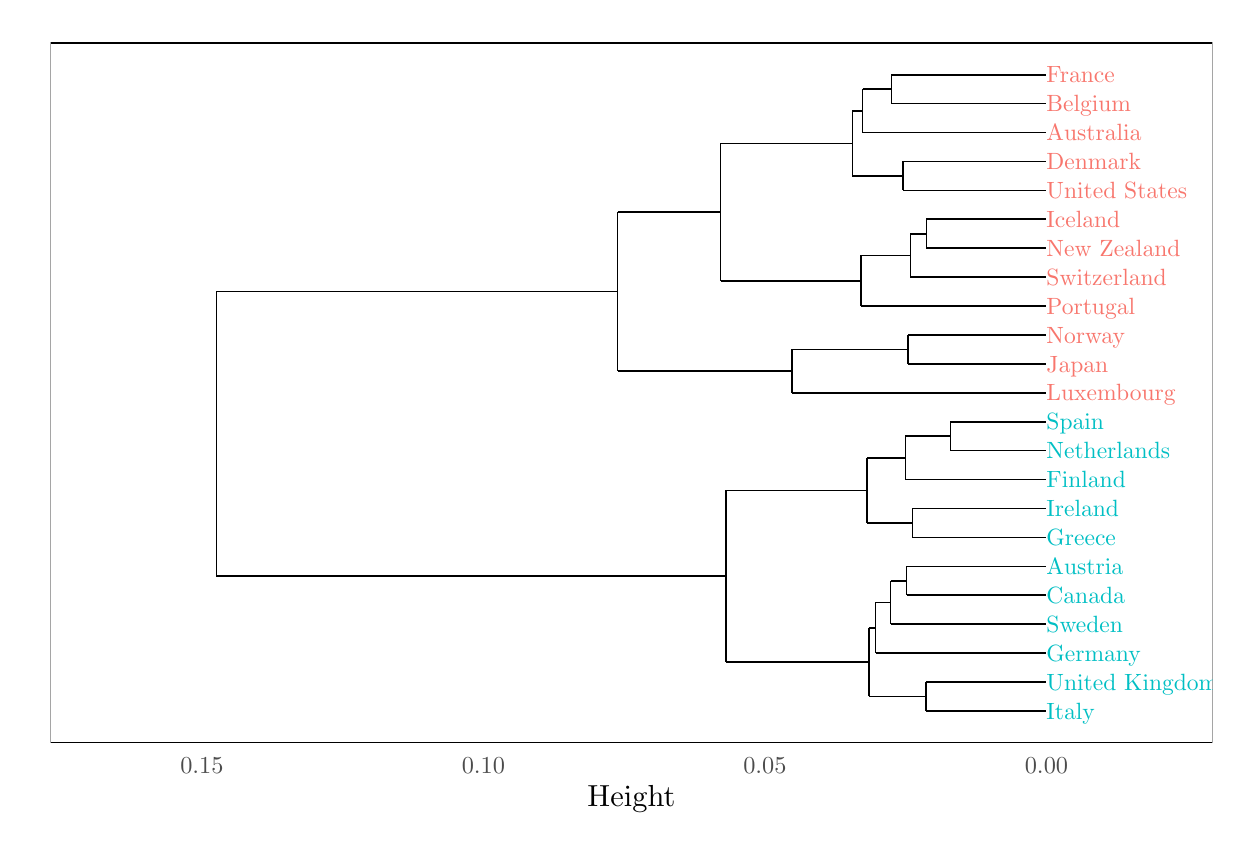
\begin{tikzpicture}[x=1pt,y=1pt]
\definecolor{fillColor}{RGB}{255,255,255}
\path[use as bounding box,fill=fillColor,fill opacity=0.00] (0,0) rectangle (433.62,289.08);
\begin{scope}
\path[clip] (  8.25, 30.69) rectangle (428.12,283.58);
\definecolor{drawColor}{RGB}{0,0,0}
\definecolor{fillColor}{RGB}{255,255,255}

\path[draw=drawColor,line width= 0.6pt,line join=round,line cap=round,fill=fillColor] (  8.25, 30.69) rectangle (428.12,283.58);

\path[draw=drawColor,line width= 0.6pt,line join=round] ( 68.23,142.27) -- ( 68.23, 90.84);

\path[draw=drawColor,line width= 0.6pt,line join=round] ( 68.23, 90.84) -- (252.23, 90.84);

\path[draw=drawColor,line width= 0.6pt,line join=round] (252.23, 90.84) -- (252.23, 59.82);

\path[draw=drawColor,line width= 0.6pt,line join=round] (252.23, 59.82) -- (303.93, 59.82);

\path[draw=drawColor,line width= 0.6pt,line join=round] (303.93, 59.82) -- (303.93, 47.41);

\path[draw=drawColor,line width= 0.6pt,line join=round] (303.93, 47.41) -- (324.57, 47.41);

\path[draw=drawColor,line width= 0.6pt,line join=round] (324.57, 47.41) -- (324.57, 42.18);

\path[draw=drawColor,line width= 0.6pt,line join=round] (324.57, 42.18) -- (368.14, 42.18);

\path[draw=drawColor,line width= 0.6pt,line join=round] (324.57, 47.41) -- (324.57, 52.63);

\path[draw=drawColor,line width= 0.6pt,line join=round] (324.57, 52.63) -- (368.14, 52.63);

\path[draw=drawColor,line width= 0.6pt,line join=round] (303.93, 59.82) -- (303.93, 72.23);

\path[draw=drawColor,line width= 0.6pt,line join=round] (303.93, 72.23) -- (306.40, 72.23);

\path[draw=drawColor,line width= 0.6pt,line join=round] (306.40, 72.23) -- (306.40, 63.08);

\path[draw=drawColor,line width= 0.6pt,line join=round] (306.40, 63.08) -- (368.14, 63.08);

\path[draw=drawColor,line width= 0.6pt,line join=round] (306.40, 72.23) -- (306.40, 81.37);

\path[draw=drawColor,line width= 0.6pt,line join=round] (306.40, 81.37) -- (311.81, 81.37);

\path[draw=drawColor,line width= 0.6pt,line join=round] (311.81, 81.37) -- (311.81, 73.53);

\path[draw=drawColor,line width= 0.6pt,line join=round] (311.81, 73.53) -- (368.14, 73.53);

\path[draw=drawColor,line width= 0.6pt,line join=round] (311.81, 81.37) -- (311.81, 89.21);

\path[draw=drawColor,line width= 0.6pt,line join=round] (311.81, 89.21) -- (317.61, 89.21);

\path[draw=drawColor,line width= 0.6pt,line join=round] (317.61, 89.21) -- (317.61, 83.98);

\path[draw=drawColor,line width= 0.6pt,line join=round] (317.61, 83.98) -- (368.14, 83.98);

\path[draw=drawColor,line width= 0.6pt,line join=round] (317.61, 89.21) -- (317.61, 94.43);

\path[draw=drawColor,line width= 0.6pt,line join=round] (317.61, 94.43) -- (368.14, 94.43);

\path[draw=drawColor,line width= 0.6pt,line join=round] (252.23, 90.84) -- (252.23,121.86);

\path[draw=drawColor,line width= 0.6pt,line join=round] (252.23,121.86) -- (303.39,121.86);

\path[draw=drawColor,line width= 0.6pt,line join=round] (303.39,121.86) -- (303.39,110.11);

\path[draw=drawColor,line width= 0.6pt,line join=round] (303.39,110.11) -- (319.67,110.11);

\path[draw=drawColor,line width= 0.6pt,line join=round] (319.67,110.11) -- (319.67,104.88);

\path[draw=drawColor,line width= 0.6pt,line join=round] (319.67,104.88) -- (368.14,104.88);

\path[draw=drawColor,line width= 0.6pt,line join=round] (319.67,110.11) -- (319.67,115.33);

\path[draw=drawColor,line width= 0.6pt,line join=round] (319.67,115.33) -- (368.14,115.33);

\path[draw=drawColor,line width= 0.6pt,line join=round] (303.39,121.86) -- (303.39,133.62);

\path[draw=drawColor,line width= 0.6pt,line join=round] (303.39,133.62) -- (317.19,133.62);

\path[draw=drawColor,line width= 0.6pt,line join=round] (317.19,133.62) -- (317.19,125.78);

\path[draw=drawColor,line width= 0.6pt,line join=round] (317.19,125.78) -- (368.14,125.78);

\path[draw=drawColor,line width= 0.6pt,line join=round] (317.19,133.62) -- (317.19,141.46);

\path[draw=drawColor,line width= 0.6pt,line join=round] (317.19,141.46) -- (333.44,141.46);

\path[draw=drawColor,line width= 0.6pt,line join=round] (333.44,141.46) -- (333.44,136.23);

\path[draw=drawColor,line width= 0.6pt,line join=round] (333.44,136.23) -- (368.14,136.23);

\path[draw=drawColor,line width= 0.6pt,line join=round] (333.44,141.46) -- (333.44,146.68);

\path[draw=drawColor,line width= 0.6pt,line join=round] (333.44,146.68) -- (368.14,146.68);

\path[draw=drawColor,line width= 0.6pt,line join=round] ( 68.23,142.27) -- ( 68.23,193.71);

\path[draw=drawColor,line width= 0.6pt,line join=round] ( 68.23,193.71) -- (213.18,193.71);

\path[draw=drawColor,line width= 0.6pt,line join=round] (213.18,193.71) -- (213.18,164.97);

\path[draw=drawColor,line width= 0.6pt,line join=round] (213.18,164.97) -- (276.22,164.97);

\path[draw=drawColor,line width= 0.6pt,line join=round] (276.22,164.97) -- (276.22,157.13);

\path[draw=drawColor,line width= 0.6pt,line join=round] (276.22,157.13) -- (368.14,157.13);

\path[draw=drawColor,line width= 0.6pt,line join=round] (276.22,164.97) -- (276.22,172.81);

\path[draw=drawColor,line width= 0.6pt,line join=round] (276.22,172.81) -- (318.21,172.81);

\path[draw=drawColor,line width= 0.6pt,line join=round] (318.21,172.81) -- (318.21,167.58);

\path[draw=drawColor,line width= 0.6pt,line join=round] (318.21,167.58) -- (368.14,167.58);

\path[draw=drawColor,line width= 0.6pt,line join=round] (318.21,172.81) -- (318.21,178.03);

\path[draw=drawColor,line width= 0.6pt,line join=round] (318.21,178.03) -- (368.14,178.03);

\path[draw=drawColor,line width= 0.6pt,line join=round] (213.18,193.71) -- (213.18,222.45);

\path[draw=drawColor,line width= 0.6pt,line join=round] (213.18,222.45) -- (250.36,222.45);

\path[draw=drawColor,line width= 0.6pt,line join=round] (250.36,222.45) -- (250.36,197.63);

\path[draw=drawColor,line width= 0.6pt,line join=round] (250.36,197.63) -- (301.20,197.63);

\path[draw=drawColor,line width= 0.6pt,line join=round] (301.20,197.63) -- (301.20,188.48);

\path[draw=drawColor,line width= 0.6pt,line join=round] (301.20,188.48) -- (368.14,188.48);

\path[draw=drawColor,line width= 0.6pt,line join=round] (301.20,197.63) -- (301.20,206.77);

\path[draw=drawColor,line width= 0.6pt,line join=round] (301.20,206.77) -- (318.96,206.77);

\path[draw=drawColor,line width= 0.6pt,line join=round] (318.96,206.77) -- (318.96,198.93);

\path[draw=drawColor,line width= 0.6pt,line join=round] (318.96,198.93) -- (368.14,198.93);

\path[draw=drawColor,line width= 0.6pt,line join=round] (318.96,206.77) -- (318.96,214.61);

\path[draw=drawColor,line width= 0.6pt,line join=round] (318.96,214.61) -- (324.78,214.61);

\path[draw=drawColor,line width= 0.6pt,line join=round] (324.78,214.61) -- (324.78,209.38);

\path[draw=drawColor,line width= 0.6pt,line join=round] (324.78,209.38) -- (368.14,209.38);

\path[draw=drawColor,line width= 0.6pt,line join=round] (324.78,214.61) -- (324.78,219.83);

\path[draw=drawColor,line width= 0.6pt,line join=round] (324.78,219.83) -- (368.14,219.83);

\path[draw=drawColor,line width= 0.6pt,line join=round] (250.36,222.45) -- (250.36,247.27);

\path[draw=drawColor,line width= 0.6pt,line join=round] (250.36,247.27) -- (297.99,247.27);

\path[draw=drawColor,line width= 0.6pt,line join=round] (297.99,247.27) -- (297.99,235.51);

\path[draw=drawColor,line width= 0.6pt,line join=round] (297.99,235.51) -- (316.38,235.51);

\path[draw=drawColor,line width= 0.6pt,line join=round] (316.38,235.51) -- (316.38,230.28);

\path[draw=drawColor,line width= 0.6pt,line join=round] (316.38,230.28) -- (368.14,230.28);

\path[draw=drawColor,line width= 0.6pt,line join=round] (316.38,235.51) -- (316.38,240.73);

\path[draw=drawColor,line width= 0.6pt,line join=round] (316.38,240.73) -- (368.14,240.73);

\path[draw=drawColor,line width= 0.6pt,line join=round] (297.99,247.27) -- (297.99,259.02);

\path[draw=drawColor,line width= 0.6pt,line join=round] (297.99,259.02) -- (301.72,259.02);

\path[draw=drawColor,line width= 0.6pt,line join=round] (301.72,259.02) -- (301.72,251.18);

\path[draw=drawColor,line width= 0.6pt,line join=round] (301.72,251.18) -- (368.14,251.18);

\path[draw=drawColor,line width= 0.6pt,line join=round] (301.72,259.02) -- (301.72,266.86);

\path[draw=drawColor,line width= 0.6pt,line join=round] (301.72,266.86) -- (312.09,266.86);

\path[draw=drawColor,line width= 0.6pt,line join=round] (312.09,266.86) -- (312.09,261.63);

\path[draw=drawColor,line width= 0.6pt,line join=round] (312.09,261.63) -- (368.14,261.63);

\path[draw=drawColor,line width= 0.6pt,line join=round] (312.09,266.86) -- (312.09,272.08);

\path[draw=drawColor,line width= 0.6pt,line join=round] (312.09,272.08) -- (368.14,272.08);
\definecolor{drawColor}{RGB}{248,118,109}

\node[text=drawColor,anchor=base west,inner sep=0pt, outer sep=0pt, scale=  0.85] at (368.14,248.24) {Australia};
\definecolor{drawColor}{RGB}{0,191,196}

\node[text=drawColor,anchor=base west,inner sep=0pt, outer sep=0pt, scale=  0.85] at (368.14, 91.49) {Austria};
\definecolor{drawColor}{RGB}{248,118,109}

\node[text=drawColor,anchor=base west,inner sep=0pt, outer sep=0pt, scale=  0.85] at (368.14,258.70) {Belgium};
\definecolor{drawColor}{RGB}{0,191,196}

\node[text=drawColor,anchor=base west,inner sep=0pt, outer sep=0pt, scale=  0.85] at (368.14, 81.04) {Canada};
\definecolor{drawColor}{RGB}{248,118,109}

\node[text=drawColor,anchor=base west,inner sep=0pt, outer sep=0pt, scale=  0.85] at (368.14,237.79) {Denmark};
\definecolor{drawColor}{RGB}{0,191,196}

\node[text=drawColor,anchor=base west,inner sep=0pt, outer sep=0pt, scale=  0.85] at (368.14,122.84) {Finland};
\definecolor{drawColor}{RGB}{248,118,109}

\node[text=drawColor,anchor=base west,inner sep=0pt, outer sep=0pt, scale=  0.85] at (368.14,269.15) {France};
\definecolor{drawColor}{RGB}{0,191,196}

\node[text=drawColor,anchor=base west,inner sep=0pt, outer sep=0pt, scale=  0.85] at (368.14, 60.14) {Germany};

\node[text=drawColor,anchor=base west,inner sep=0pt, outer sep=0pt, scale=  0.85] at (368.14,101.94) {Greece};
\definecolor{drawColor}{RGB}{248,118,109}

\node[text=drawColor,anchor=base west,inner sep=0pt, outer sep=0pt, scale=  0.85] at (368.14,216.89) {Iceland};
\definecolor{drawColor}{RGB}{0,191,196}

\node[text=drawColor,anchor=base west,inner sep=0pt, outer sep=0pt, scale=  0.85] at (368.14,112.39) {Ireland};

\node[text=drawColor,anchor=base west,inner sep=0pt, outer sep=0pt, scale=  0.85] at (368.14, 39.24) {Italy};
\definecolor{drawColor}{RGB}{248,118,109}

\node[text=drawColor,anchor=base west,inner sep=0pt, outer sep=0pt, scale=  0.85] at (368.14,164.64) {Japan};

\node[text=drawColor,anchor=base west,inner sep=0pt, outer sep=0pt, scale=  0.85] at (368.14,154.19) {Luxembourg};
\definecolor{drawColor}{RGB}{0,191,196}

\node[text=drawColor,anchor=base west,inner sep=0pt, outer sep=0pt, scale=  0.85] at (368.14,133.29) {Netherlands};
\definecolor{drawColor}{RGB}{248,118,109}

\node[text=drawColor,anchor=base west,inner sep=0pt, outer sep=0pt, scale=  0.85] at (368.14,206.44) {New Zealand};

\node[text=drawColor,anchor=base west,inner sep=0pt, outer sep=0pt, scale=  0.85] at (368.14,175.09) {Norway};

\node[text=drawColor,anchor=base west,inner sep=0pt, outer sep=0pt, scale=  0.85] at (368.14,185.54) {Portugal};
\definecolor{drawColor}{RGB}{0,191,196}

\node[text=drawColor,anchor=base west,inner sep=0pt, outer sep=0pt, scale=  0.85] at (368.14,143.74) {Spain};

\node[text=drawColor,anchor=base west,inner sep=0pt, outer sep=0pt, scale=  0.85] at (368.14, 70.59) {Sweden};
\definecolor{drawColor}{RGB}{248,118,109}

\node[text=drawColor,anchor=base west,inner sep=0pt, outer sep=0pt, scale=  0.85] at (368.14,195.99) {Switzerland};
\definecolor{drawColor}{RGB}{0,191,196}

\node[text=drawColor,anchor=base west,inner sep=0pt, outer sep=0pt, scale=  0.85] at (368.14, 49.69) {United Kingdom};
\definecolor{drawColor}{RGB}{248,118,109}

\node[text=drawColor,anchor=base west,inner sep=0pt, outer sep=0pt, scale=  0.85] at (368.14,227.34) {United States};
\end{scope}
\begin{scope}
\path[clip] (  0.00,  0.00) rectangle (433.62,289.08);
\definecolor{drawColor}{gray}{0.30}

\node[text=drawColor,anchor=base,inner sep=0pt, outer sep=0pt, scale=  0.88] at (368.14, 19.68) {0.00};

\node[text=drawColor,anchor=base,inner sep=0pt, outer sep=0pt, scale=  0.88] at (266.41, 19.68) {0.05};

\node[text=drawColor,anchor=base,inner sep=0pt, outer sep=0pt, scale=  0.88] at (164.69, 19.68) {0.10};

\node[text=drawColor,anchor=base,inner sep=0pt, outer sep=0pt, scale=  0.88] at ( 62.97, 19.68) {0.15};
\end{scope}
\begin{scope}
\path[clip] (  0.00,  0.00) rectangle (433.62,289.08);
\definecolor{drawColor}{RGB}{0,0,0}

\node[text=drawColor,anchor=base,inner sep=0pt, outer sep=0pt, scale=  1.10] at (218.18,  7.64) {Height};
\end{scope}
\end{tikzpicture}
